% LaTeX template for reports
% Author: Adam Jaamour
% Last updated: 13/04/2020

% ------------------- IMPORTS -------------------
\documentclass[letterpaper,12pt]{article}
\usepackage{tabularx} % extra features for tabular environment
\usepackage{amsmath}  % improve maths presentation
\usepackage{amssymb} % maths symbols
\usepackage{graphicx} % takes care of graphic including machinery
\usepackage[margin=0.95in,letterpaper]{geometry} % decreases margins
\usepackage{cite} % takes care of citations
\usepackage[titletoc,title]{appendix} % takes care of appendices
\usepackage{listings} % code representation
\usepackage{pdflscape}
\usepackage{csquotes} % for quoting existing work
\usepackage{color} % defines colours for code listings
\usepackage{comment} % allows for block of comments
\usepackage{textcomp, gensymb} % degree symbol
\usepackage[table,xcdraw]{xcolor} % table colouring
\usepackage[cc]{titlepic}  % allows a pic to be included in the title page
\usepackage[final]{hyperref} % adds hyper links inside the generated pdf file
\usepackage{pdfpages} % include pdfs
\usepackage{subcaption} % subfigures to have multiple images on the same line

% ------------------- CODING STYLE -------------------
\definecolor{codegreen}{rgb}{0,0.6,0}
\definecolor{codegray}{rgb}{0.5,0.5,0.5}
\definecolor{backcolour}{rgb}{0.95,0.95,0.92}
\lstdefinestyle{mystyle}{
    backgroundcolor=\color{backcolour},   
    commentstyle=\color{codegreen},
    keywordstyle=\color{blue},
    numberstyle=\tiny\color{codegray},
    basicstyle=\footnotesize,
    breakatwhitespace=false,         
    breaklines=true,                 
    captionpos=b,                    
    keepspaces=true,                 
    numbersep=5pt,                  
    showspaces=false,                
    showstringspaces=false,
    showtabs=false,                  
    tabsize=4
}
\lstset{style=mystyle}

% ------------------- HEADINGS -------------------

\begin{document}

\title{
    CS5014 Machine Learning\\Practical 2 Report\\
    \begin{large}
    University of St Andrews - School of Computer Science
    \end{large}
}
\titlepic{
\includegraphics[width=0.3\linewidth]{figures/st-andrews-logo.jpeg}}
\author{Student ID: 150014151}
\date{5th May, 2020}
\maketitle
\newpage

\tableofcontents
\newpage

% ------------------- INTRODUCTION --------------------

\section{Introduction}
\label{sec:introduction}

This practical covers the exploration of various machine learning practices used when dealing with real-life data. The data in question documents different types of seal pups found in cropped aerial imagery obtained during seasonal surveys of islands. Various data visualisation techniques, data processing steps and classification models are experimented with to design a final pipeline for making predictions on the types of seals observed in the images. The predictions are made by training multiple classification models, which are all evaluated to determine their performance.\\

The report is separated in four sections, starting with a general introductory section before exploring the diverse array of methodologies and design decisions made during the development of the code in Python, followed by an evaluation of the final classifier and a critical reflection on the findings.

\subsection{Usage instructions}

Before running the code, create a new virtual environment and install the Python libraries used in the code by running the following command:

\begin{lstlisting}
pip install -r requirements.txt
\end{lstlisting}

To run the program, move to the “src” directory and run the following command:

\begin{lstlisting}
python main.py -s <section> -d <dataset> [-m <model>] [-g] [-v]
\end{lstlisting}

where:
\begin{itemize}
    \item``\textit{-s section}'': is a setting that executes different parts of the program. It must be one of the following: `\textit{data\_vis}', `\textit{train}' or `\textit{test}'.
    \item``\textit{-d dataset}'': selects the dataset to use. It must be set to either `\textit{binary}' or `\textit{multi}'.
    \item``\textit{-m model}'': is an optional setting that selects the classification model to use for training. It must be one of the following: `\textit{sgd}', `\textit{logistic}', `\textit{svc\_lin}', `\textit{svc\_poly}'.
    \item``\textit{-gs}'' and ``\textit{-gs}'': are optional flags to run the hyperparameter tuning algorithms (either grid search or randomised search algorithms) for the selected classification model. The flag only takes effect when using multi-layer perceptron classifiers (neural networks).
    \item``\textit{-v}'': is an optional flag that enters verbose (debugging) mode, printing additional statements on the command line.
\end{itemize}

\subsection{Tools used}

\begin{itemize}
    \item Programming language: Python 3.7.
    \item Python libraries used: SciKit-Learn \cite{scikit-learn}, Pandas \cite{reback2020pandas}, Matplotlib \cite{Hunter:2007}, NumPy \cite{numpy},  Seaborn \cite{seaborn} and Imbalanced-Learn \cite{JMLR:v18:16-365}.
    \item Editor: PyCharm\footnote{PyCharm: \url{https://www.jetbrains.com/pycharm/}}.
    \item Version controlling: Git and GitHub (private repository).
    \item Initial code prototyping: Jupyter Lab.
\end{itemize}

% ------------------- SYSTEM ARCHITECTURE --------------------

\section{System Architecture}
\label{sec:system-architecture}

\subsection{Project structure}

The project is organised into the following python modules:
\begin{itemize}
    \item `\textit{main.py}': 
    \item `\textit{data\_visualisation.py}': 
    \item `\textit{data\_manipulations.py}': 
    \item `\textit{classifiers.py}':
    \item `\textit{helpers.py}': 
    \item `\textit{config.py}': 
\end{itemize}

\subsection{Execution flow}

A command-line interface, implemented through Python’s native library \textit{argparse}\footnote{argparse: \url{https://docs.python.org/3.7/library/argparse.html}}, controls which dataset to use and which part of the program to run:
\begin{itemize}
    \item Visualising the data sets.
    \item Training different classification models.
    \item Running a hyperparameter tuning algorithm (grid search or randomised search) on promising models.
    \item Making predictions using the final model.
\end{itemize}

% ------------------- PART 3: Methodology, design decisions --------------------

\section{Methodology \& data-driven design decisions}
\label{sec:methodology-design}

\subsection{Datasets}

\subsubsection{Data description}

The data comes in two flavours: \textit{binary} and \textit{multi}, where the ``\textit{binary}'' data contains two labels, one for images of backgrounds and the other images of seals, and  the ``\textit{multi}'' data contains five labels, one for images of backgrounds and the four others for types of seals (whitecoat, moulted pup, dead pup and juvenile).

\subsubsection{Data loading}
\label{sec:data-loading}

Each dataset contains three distinct CSV files:
\begin{itemize}
    \item ``\textit{X\_train.csv}'', containing the features describing the images, which are analysed in further sections.
    \item ``\textit{Y\_train.csv}'', containing the class/label for each image.
    \item ``\textit{X\_test.csv}'', containing the features of the images to test. These are used for making the final predictions with the optimal trained classifier.
\end{itemize}

The provided CSV files are directly loaded into distinct Pandas DataFrames\footnote{Pandas DataFrames: \url{https://pandas.pydata.org/pandas-docs/stable/reference/api/pandas.DataFrame.html}} by using the \textit{read\_csv} function. However, this method takes a long time due to the large file size (e.g. X\_train.csv is 1.5GB large). To speed up the process, the DataFrames are therefore serialised and saved using Pickle\footnote{Pickle: \url{https://docs.python.org/3.7/library/pickle.html}}, boosting future loading times from 11.3 to 0.6 seconds.

% -------------------

\subsection{Data visualisation \& Analysis}

This data visualisation step\footnote{Note: running the code to visualise all the figures and tables produced takes roughly 80 seconds.} is crucial to understand the data and its underlying patterns before fitting a classification model to the training data.

\subsubsection{Data overview}

Storing the features and labels in a \textit{DataFrames} provides a valuable array of functions that can be used to gain high-level insights on the data. Using the \textit{pandas.DataFrame.info} and \textit{pandas.DataFrame.describe} functions reveals important information such as:
\begin{itemize}
    \item There are 62210 samples in the training set, each described by 964 features (columns).
    \item There are no missing values in the entire dataset as each feature has 62210 non-null values (number of images in the training set).
    \item All training values are numerical (floats).
\end{itemize}

This initial overview confirms that no data encoding is required to use the features, and that the data is considered to ``clean'', thus requiring no processing.

\subsubsection{Classes distribution}
\label{sec:classes-distribution}

s this is a classification task, it is important to verify the distribution of classes in the training  set to determine whether the data is skewed or not (whether some classes are much more frequent than other classes \cite{Geron2019}). This is achieved by plotting the labels found in ``\textit{Y\_train.csv}'' in bar charts (see Figure \ref{fig:class_distribution}).\\

\begin{figure}[h]
\centering
\begin{subfigure}{.5\textwidth}
  \centering
  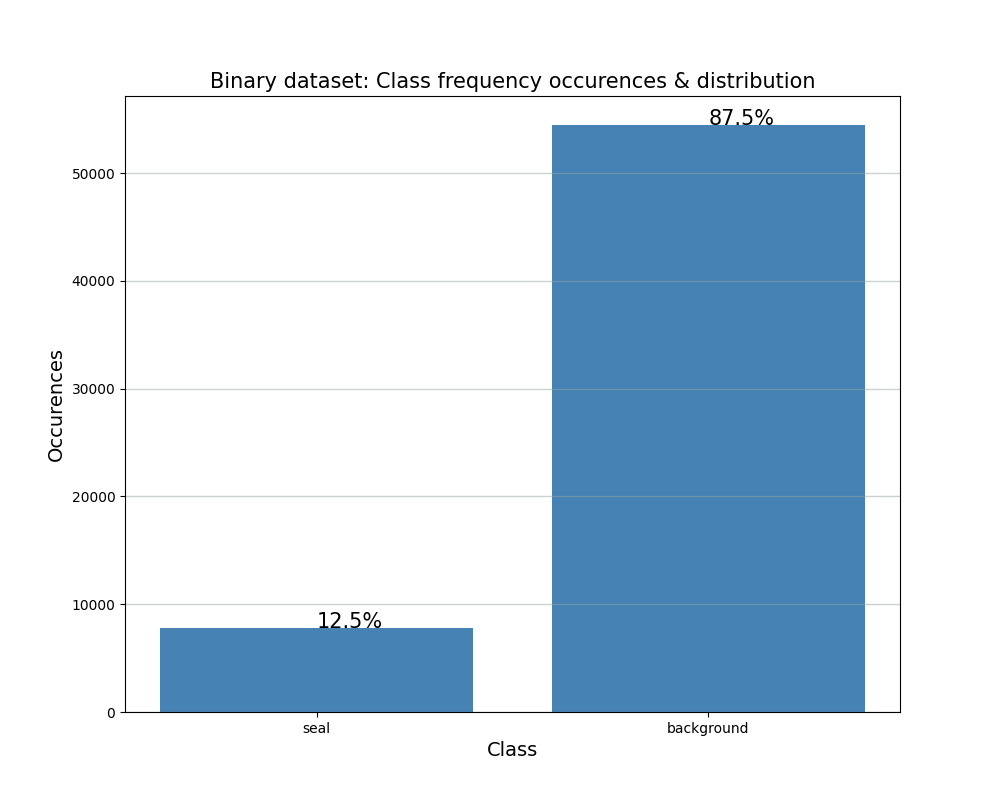
\includegraphics[width=\textwidth]{results/binary_class_distribution.png}
  \label{fig:binary_class_distribution}
\end{subfigure}%
\begin{subfigure}{.5\textwidth}
  \centering
  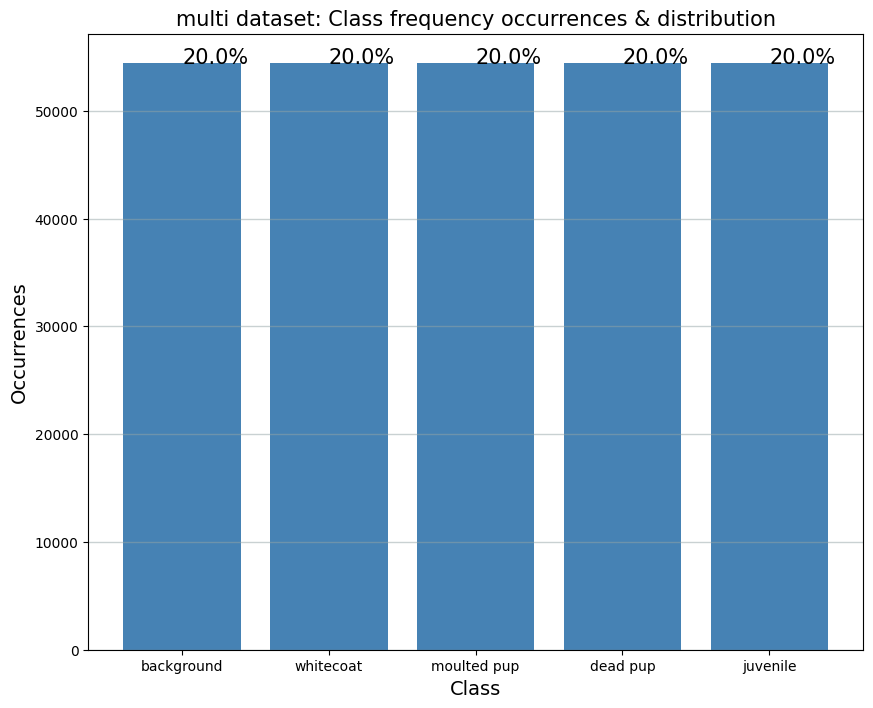
\includegraphics[width=\textwidth]{results/multi_class_distribution.png}
  \label{fig:multi_class_distribution}
\end{subfigure}
\caption{\label{fig:class_distribution}Class distribution of the binary (left) and multi (right) datasets.}
\end{figure}

These bar charts reveal that both datasets are heavily unbalanced, which must be taken into account when analysing the classifiers' scores. Indeed, using an  evaluation metric such as accuracy would be misleading as it would not be representative of how well the classifier fitted the data. For instance, if a dumb classifier that always classified an image as ``background'' was created, it would achieve 87.5\% accuracy on the binary dataset. Therefore, other metrics such as confusion matrices, precision, recall and F1 scores could be used \cite{Geron2019}. These are further explored in Section \ref{sec:performance-metrics}. A potential solution to counter the imbalance would be to oversample the dataset \cite{becker2020}.

\subsubsection{Features \& correlation}

There are three different types of features describing each image (row) in the datasets:
\begin{itemize}
    \item \textit{Histogram of oriented Gradients (HoG)}, which correspond to a type of feature often used in computer vision. These extracting HoGs are histograms counting the occurrences of gradient orientations (9 orientations) in 2x2 blocks \cite{Dalal2005}. In the ``\textit{X\_train.csv}'' datasets, they correspond to the first 900 columns.
    \item \textit{Samples from a normal distribution} with parameters $\mu=0.5$ and $\sigma=2$. These correspond to columns 900 to 916 amongst the features dataset.
    \item 16-bin \textit{RGB colour histograms}, corresponding to the last 48 columns in the features dataset.
\end{itemize}

Not all 964 features should be used due to the large complexity introduced by the number of dimensions the data has, also known as the curse of dimensionality \cite{Geron2019}. A preliminary check to determine which features can be considered ``important'' is conducted by calculating the standard correlation coefficient, a value ranging between -1 and 1, between the labels in (``\textit{Y\_train.csv}'') and all the features ``\textit{X\_train.csv}''. A value close to 1 indicates a strong positive linear correlation, while a correlation close to -1 indicates a strong negative linear correlation. However, a correlation close to 0 indicates a lack of relationship in the data. According to existing literature, features are considered to have a high correlation when they have values in the region of $[|0.5,0.7|]$ \cite{Geron2019} \cite{Badr2019}. To determine which features show the highest correlation with the class labels, the \textit{pandas.DataFrame.corr} function is used on a concatenated DataFrame of the features and the labels. The ten features with the highest positive and negative correlation are shown in Figure \ref{fig:correlation-results}.

\begin{figure}[h]
\centering
\begin{subfigure}{.49\textwidth}
  \centering
  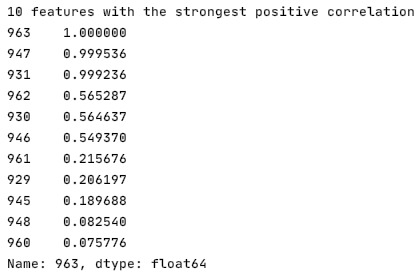
\includegraphics[width=\textwidth]{report/figures/corr_pos.png}
  \label{fig:corr_pos}
\end{subfigure}%
\begin{subfigure}{.5\textwidth}
  \centering
  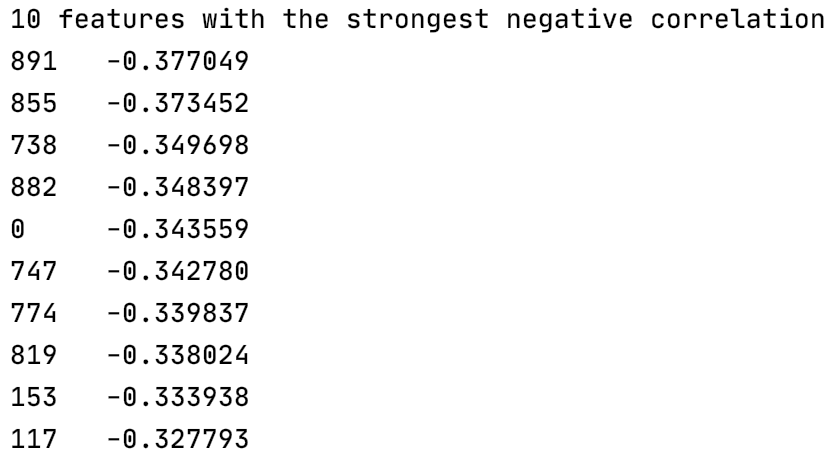
\includegraphics[width=\textwidth]{report/figures/corr_neg.png}
  \label{fig:corr_neg}
\end{subfigure}
\caption{\label{fig:correlation-results}Top 10 training dataset column indexes (features) with the highest standard correlation coefficient. Left shows positive correlations, right shows negative correlation.}
\end{figure}

High positive correlation is achieved for features ranging between columns 916-964, which corresponds to RGB colour histograms, while high negative correlation is achieved for features ranging between columns 0-900, which corresponds to HoGs. However, because no feature from the normal distribution have a high correlation  with the class labels, it can be dropped altogether.

\subsubsection{Visualising features}

\paragraph{HoG features}

To directly visualise some information about the images, the HoG features are reconstructed into images by being reshaped into 30x30 images, as seen in Figure \ref{fig:hog_multi}. Visualising the reconstructed HoG images confirms how it is impossible to discern the different classes with the human eye alone, and depicts how it will be impossible to infer anything from the reconstructed images of misclassified predictions.

\begin{figure}[h]
\centerline{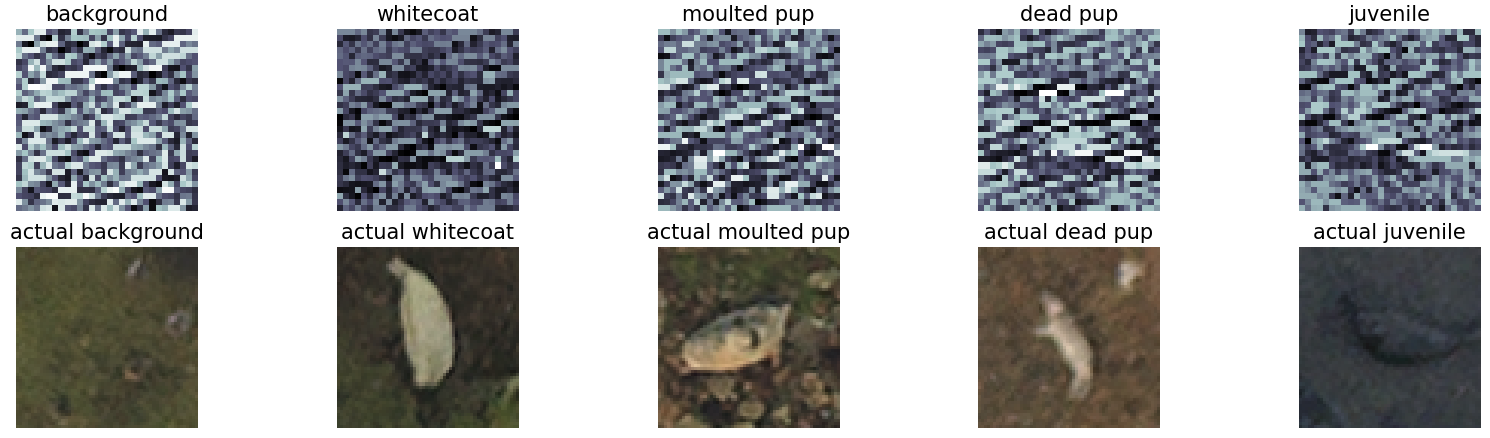
\includegraphics[width=\textwidth]{report/figures/hog_multi.png}}
\caption{\label{fig:hog_multi}Comparison of images reconstructed images from HoG features (top and middle rows) with actual images (bottom row).}
\end{figure}

\paragraph{RGB colour histograms}

The features corresponding to the RGB colour histograms are visualised in Figure \ref{fig:rgb-hists}, revealing that there are more low-intensity pixels than high-intensity pixels.\\

Due to the considerable spread across the x and y axes witnessed in the range of values for HoGs and RGB histograms (data distribution is not bell-shaped  as some values are more concentrated on extremities, and ) the data will require some feature transformation such as standardising the dataset.

\begin{figure}[h]
\centering
\begin{subfigure}{.41\textwidth}
  \centering
  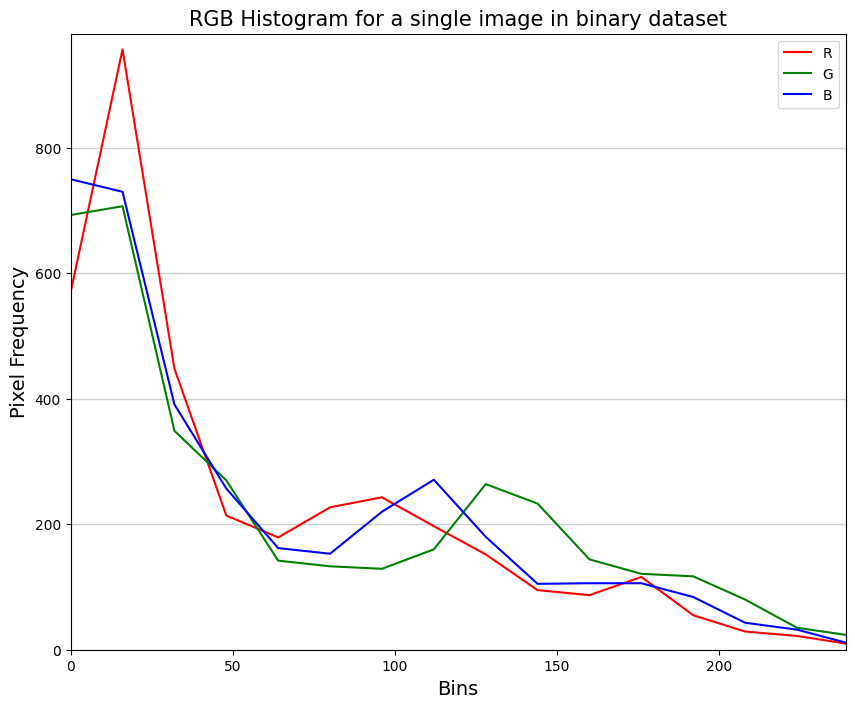
\includegraphics[width=\textwidth]{results/rgb_hist_single_image_binary.png}
  \label{fig:rgb_hist_single_image_binary}
\end{subfigure}%
\begin{subfigure}{.5\textwidth}
  \centering
  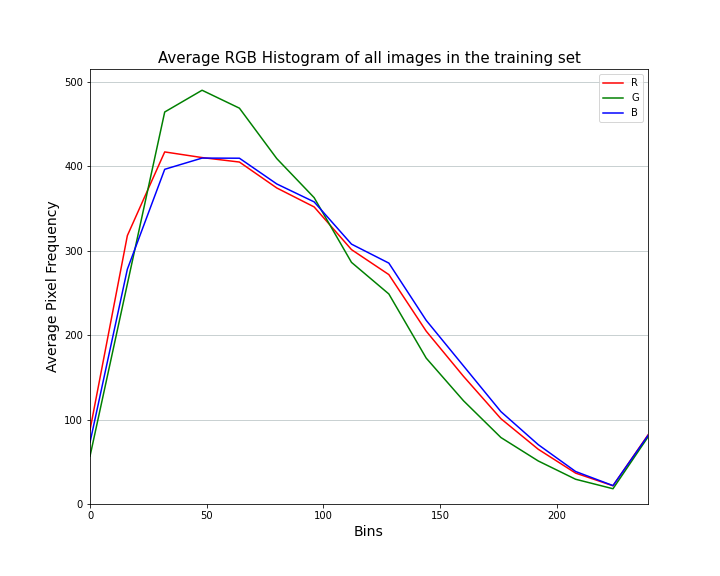
\includegraphics[width=\textwidth]{jupyter prototyping/rgb_avg_hist_all_training_set.png}
  \label{fig:rgb_avg_hist_all_training_set}
\end{subfigure}
\caption{\label{fig:rgb-hists}RGB histogram for a single random image (left) and average of all images in the training set (right).}
\end{figure}

% -------------------

\newpage
\subsection{Data pre-processing}
\label{sec:data-preprocessing-steps}

With the data visualisation and analysis steps completed, the training set can now be pre-processed to optimise the classification models’ fit on the data. Based on the conclusions made from the data analysis, three pre-processing steps are carried out.

\subsubsection{Step 1: SMOTE oversampling}

todo

classes distribution Section \ref{sec:classes-distribution}

\subsubsection{Step 2: Dropping features with poor correlation}
\label{sec:drop-poor-features}

Based on the correlation results, the normal distribution features can be dropped from the training dataset. This brings down the number of dimensions in the training data from 964 to 948.\\

\subsubsection{Step 3: Standardising the dataset}
\label{sec:standard-scaling}

Next, visualising the values of the dataset revealed how the data distribution is not bell-shaped and has very different scales between the HoG features and the RGB histograms. Therefore, the features are standardised using the \textit{sklearn.preprocessing.StandardScaler} class, resulting in a distribution with unit variance a shape closer to a bell (the two properties of standardised distributions are a mean of all values equal to 0 and a standard deviation equal to 1) \cite{Geron2019}\cite{Glen2014}. The \textit{StandardScaler} instance used is saved to a Pickle file in the ``\textit{transform\_pipeline}'' directory to eventually apply the same the transformations on the test data.

\subsubsection{Step 4: Principal Component Analysis}
\label{sec:pca}

However, the curse of dimensionality remains as there are still 948 columns in the dataset. The most popular solution to counter this problem is to use Principal Component Analysis (PCA) to reduce the number of dimensions via projection. This is achieved by using the \textit{sklearn.decomposition.PCA} class. In order to choose the right number of dimensions to keep to preserve 99\% of the training set's explained variance, the explained variance is plotted against the number of dimensions in Figure \ref{fig:explained_variance}. The plot shows that to maintain 99\% variance in the binary dataset, 492 dimensions can be kept (Figure \ref{fig:explained_variance_binary}), while 475 dimensions can be kept in the multi dataset (Figure \ref{fig:explained_variance_multi}). Diminishing the number of dimensions any lower would reduce the variance under 99\% \cite{Geron2019}. The training set is therefore reduced to almost half the size of the original dataset. The \textit{PCA} instance used is also saved to a Pickle file in the ``\textit{transform\_pipeline}'' directory to apply the same the dimension reduction on the test data.

\begin{figure}[h]
\centering
\begin{subfigure}{0.5\textwidth}
  \centering
  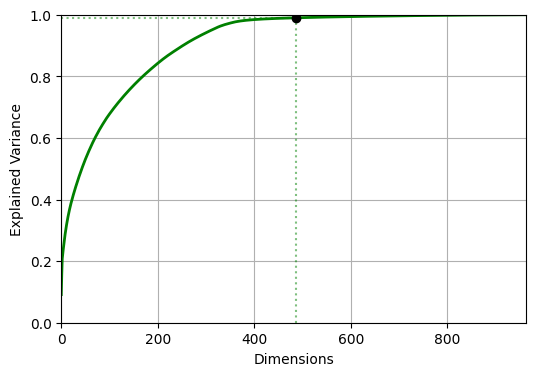
\includegraphics[width=\textwidth]{report/figures/explained_variance_multi.png}
  \caption{Binary dataset: 492 dimensions.}
  \label{fig:explained_variance_binary}
\end{subfigure}%
\begin{subfigure}{.5\textwidth}
  \centering
  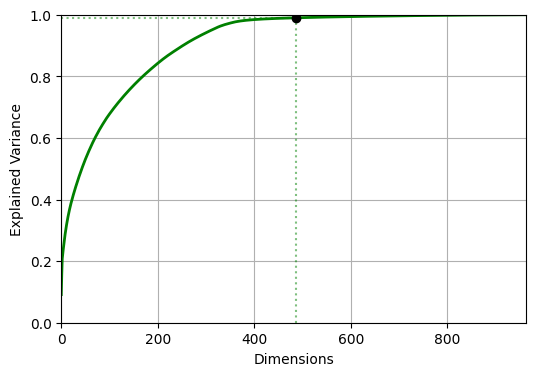
\includegraphics[width=\textwidth]{report/figures/explained_variance_multi.png}
    \caption{Multi dataset: 475 dimensions.}
  \label{fig:explained_variance_multi}
\end{subfigure}
\caption{\label{fig:explained_variance}Explained variance plotted against number of dimensions to reveal the number of dimensions that are  required to maintain 99\% variance in both datasets.}
\end{figure}

\subsubsection{Step 5: Label prepration}

todo

% -------------------

\subsection{Model Training}

\subsubsection{Model selection strategy}

At this point, the training data is ready to be fed into the classifiers. The classification models will fit the features found in ``\textit{X\_train.csv}'' before making their own predictions, which will be compared with the real labels found in ``\textit{Y\_train.csv}'' for evaluation.\\

According to A. Géron, an efficient approach to model selection is to try out multiple classifiers, with hyperparameters close to the default values recommended by Scikit-Learn. The goal of this method is to gain a high-level intuition of which classification models to further explore and tweak \cite{Geron2019}.\\

After briefly evaluating a Stochastic Gradient Descent (SGD) classifier, One-verus-Rest (OvR) Logistic Regression, Linear and Polynomial (3rd degree) Support Vector Classifiers (SVC), Decision Tree and Multi Layer Perceptron\footnote{Multi Layer Perceptron are also known as Neural Networks} (MLP), using 3-fold cross validation, the MLP was selected due to its consistency across different scoring methods and its lower runtime. ``Simpler'' models such as the SGD or OvR logistic regressor were not customisable enough, running the risk of poorly adapting to the large dataset, whereas Support  Vector Machine-based and Decision Tree-based classifiers took a very long time to fit and  are likely to overfit the data if poorly tuned. Therefore, neural networks provided the perfect middle ground for being highly customisable (23 hyperparameters) and quicker than the other models. See Appendix \ref{sec:appendix-initial-default-classifiers} for the results in tabular format.

\subsubsection{Classification performance metrics}
\label{sec:performance-metrics}

As mentioned earlier in Section \ref{sec:classes-distribution}, simply using accuracy can be misleading. Therefore, other metrics are used, namely the F1 score and confusion matrices.

\subsubsection{K-fold cross validation}

K-fold cross validation consists of a representative way of evaluating the trained regression model. It divides the training set in $K$ subsets (e.g. K=3) and evaluates the model $K$ times. Using the \textit{sklearn.model\_selection.cross\_val\_predict} function, predictions can be made on each subset, ultimately resulting in a clean prediction for each sample in the training set (the predictions are made by a model that never saw the data during training) \cite{Geron2019}. Despite the advantages of running k-fold cross validation, it is not always possible due to the expensive cost of multiplying the runtimes by the number of folds.\\

With the research made on the use of cross validation through the \textit{cross\_val\_predict} function, the motivation to not split the training data into training/validation sets was made. Indeed, splitting  the the imbalanced training dataset using the popular 80\%/20\% split would have considerably diminished the number of samples  in infrequent classes, giving the pre-processing algorithms and classification models even less samples to learn these rare classes. For example, the ``\textit{juvenile}'' class samples would be lowered from XXX to XXX in the training dataset, which would affect the SMOTE oversampling and perhaps the models' correctness.\\

Additionally, the multi layer perceptron classifiers being the quickest  models  support the choice of using cross validation (i.e. it would have been unrealistic to use cross  validation with a polynomial SVC). Validation sets are usually created to ensure that the model can generalise to unseen data  \cite{Geron2019}, but the use of the \textit{cross\_val\_predict} function which allows clean predictions to be made and detailed analysis using the metrics mentioned in Section \ref{sec:performance-metrics}, couple with the availability of the online leaderboards tool provided to view the overall accuracy of the final model's predictions made on ``\textit{X\_test.csv}'' are enough to determine if the model generalises well to unseen data.

\subsubsection{Neural network hyperparameter tuning}

The hyperparameters of Scikit-Learn’s neural network classifier class \textit{sklearn.neural\_network.MLPClassifier} are manually tried out to briefly evaluate which have an impact on the evaluation. Next, two hyperparameter tuning algorithms are run to converge towards optimal classifiers for each dataset. An initial \textit{randomised search} algorithm is run to shortlist hyperparameters that work well through the \textit{sklearn.model\_selection.RandomizedSearchCV} class. This algorithm is first chosen due to the large hyperparameter space of neural networks \cite{Geron2019}. Next, the neural network is fine-tuned with the promising hyperparameters found from the randomised search by running a grid search algorithm through the \textit{sklearn.model\_selection.GridSearchCV} class. The randomised search evaluate the model using cross-validation with random hyperparameter values, while the grid search evaluates the model with all possible combinations of hyperparameters that are specified, making it the most efficient way of fine-tuning the regression models as manually finding and testing different combinations of parameters is very time-consuming \cite{Geron2019}. The following combinations are explored using randomised and grid search, resulting in over XXX models evaluated:

\begin{lstlisting}[language=Python]
# Initialise Grid Search.
if config.is_grid_search:
    if config.dataset == "binary":
        parameters = {
            "hidden_layer_sizes": [(98,), (98, 98), (114,), (114, 114)],
            "learning_rate_init": [0.001, 0.03, 0.04, 0.1],
            "alpha": [0.0001, 0.26, 0.96]
        }
    elif config.dataset == "multi":
        parameters = {
            "hidden_layer_sizes": [(68,), (68, 68), (100,), (100, 100)],
            "learning_rate_init": [0.001, 0.01, 0.1],
            "momentum": [0.1, 0.9],
            "alpha": [0.0001, 0.1, 0.9]
        }
    searchCV = GridSearchCV(param_grid=parameters, estimator=self.clf, cv=self.folds, scoring=scoring)
# Initialise Randomised Search.
elif config.is_randomised_search:
    parameters = {
        'hidden_layer_sizes': (sp_randint(1, 150)),
        'learning_rate_init': sp_uniform(0.001, 1),
        'momentum': sp_uniform(0.1, 0.9),
        'alpha': sp_uniform(0.0001, 1)
    }
    searchCV = RandomizedSearchCV(param_distributions=parameters, estimator=self.clf, n_iter=100, cv=self.folds, scoring=scoring)
gs_results = searchCV.fit(self.X, self.y)

\end{lstlisting}

The results are all reported back into CSV files containing information about each combination of hyperparameters. The various models evaluated using  3-fold cross validation are ranked by their F1 score to determine how well the hyperparameters worked on them. The full results of each search are stored in csv files in the ``\textit{results/grid\_search}'' directory.

\subsubsection{Full training approach}
\label{sec:full-training-approach}

Training is tackled as follows:
\begin{enumerate}
    \item The dataset's features and labels (either the binary of multi) are loaded into memory (see  Section \ref{sec:data-loading}).
    \item The features are pre-processed according to the steps mentioned in Section\ref{sec:data-preprocessing-steps}, which include oversampling (for the binary dataset only), dropping features with low correlation, standardising the data and applying a PCA projection  to reduce the number of dimensions. The labels are processed as well.
    \item An instance of the custom class \textit{Classifier} is created, in which either:
    \begin{itemize}
        \item a hyperparameter-tuning algorithm is run and its results are analysed in Excel.
        \item a classification model is created based on the hyperparameter-tuning algorithm results, fitted and evaluated using cross validation and multiple performance metrics. The model is saved in a Pickle file for future reference and for the final testing phase in the directory ``\textit{trained\_classifiers}''.
    \end{itemize}
\end{enumerate}

% ------------------- CONCLUSION --------------------

\section{Conclusion: Evaluation \& Critical Discussion}
\label{sec:evaluation}

\subsection{Selecting the best classifier}

The training execution flow mentioned in Section \ref{sec:full-training-approach} is followed for both the binary and multi datasets. The table below documents the cross-validation performances for the two neural networks trained for each dataset:

todo add cross-validation scores achieved for binary and multi in a table


% This table indicates that there is minimal difference between the performance of each optimal linear regression model. Indeed, looking at the column of the optimal hyperparameters used for each optimal model, the alpha constant, which sets the strength of the regularisation for the Ridge and Lasso models, and therefore the penalty applied to irrelevant features, are near 0. This means that a general linear regression model without regularisation is actually being applied in all three cases. To break the tie, the linear regression model with Ridge regularisation is used as it includes some minor form of regularisation which may help generalise to unseen data.

\subsection{Final test}

Finally, the test features are loaded memory in the same fashion the training data was. The same data transformations that were applied to the training data are applied to the testing data, namely dropping low correlation features (see Section \ref{sec:drop-poor-features}), standardising and applying a PCA projection. This is achieved by loading back the \textit{StandardScaler} (see Section \ref{sec:standard-scaling}) and \textit{PCA} (see Section \ref{sec:pca}) instances that initially learned the training data to transform the test data. The ``\textit{transform}'' function is used rather than the ``\textit{fit\_transform}'' function to do so.\\

The predictions made on the testing data  found in ``\textit{X\_test.csv}'' are saved into a new  CSV file named ``\textit{Y\_test.csv}'', one for each  dataset. The binary and multi prediction files are uploaded to the online leaderboards tool provided  in order to get the final accuracy of the neural network:

todo add results here


\subsection{Critical discussion}

todo

% SVC and logistic regression  don't natively work with multilabel classification, whereas SGD does.

% note: performing grid search on normally processed data, then feeding the oversampled data during cross validation will largely overfit the data. As a test, this classifier was used on the testing data and uploaded on the leaderboards website, resulting in 33\% accuracy only, confirming that the model overfit the data.

% best NN based on NN without oversampling gives 93.21\% accuracy using cross validation.

% multi data set oversampling overfits data (over 97\% in cross validation, 22\% accuracy on test data)

% -------------------- APPENDIX --------------------

\begin{appendices}

\clearpage

\bibliographystyle{unsrt}
\bibliography{bibliography}

% --------------------

\clearpage
\section{Project Structure}
\label{sec:appendix-project-structure}

A screenshot of the project's file structure in the PyCharm IDE to illustrate the Python modules and data organisation.

add screenshot

% ------------------------

\clearpage
\section{Initial Default Classifiers}
\label{sec:appendix-initial-default-classifiers}

% Please add the following required packages to your document preamble:
% \usepackage{graphicx}
\begin{table}[h]
\centering
\resizebox{\textwidth}{!}{%
\begin{tabular}{|c|c|c|c|c|c|c|}
\hline
\textbf{Model} & \textbf{SGD*} & \textbf{\begin{tabular}[c]{@{}c@{}}Logistic* \\ (OvR)\end{tabular}} & \textbf{\begin{tabular}[c]{@{}c@{}}Linear \\ SVC\end{tabular}} & \textbf{\begin{tabular}[c]{@{}c@{}}Polynomial \\ SVC*\end{tabular}} & \textbf{\begin{tabular}[c]{@{}c@{}}Decision \\ Tree\end{tabular}} & \textbf{\begin{tabular}[c]{@{}c@{}}Neural \\ Network\end{tabular}} \\ \hline
\textbf{Accuracy} & 95.88\% & 96.62\% & 95.89\% & 31.58\% & 92.58\% & 93.59\% \\ \hline
\textbf{Precision} & 87.42\% & 91.14\% & 87.22\% & 14.96\% & 70.63\% & 75.98\% \\ \hline
\textbf{Recall} & 78.27\% & 80.86\% & 78.70\% & 95.46\% & 69.59\% & 71.28\% \\ \hline
\textbf{F1 score} & 82.59\% & 85.69\% & 82.74\% & 25.87\% & 70.11\% & 73.55\% \\ \hline
\textbf{\begin{tabular}[c]{@{}r@{}}Runtime \\ (seconds)\end{tabular}} & 70.28 & 104.41 & 160.09 & 252.95 & 442.02 & 13.58 \\ \hline
\textbf{\begin{tabular}[c]{@{}r@{}}Max \# \\ iterations\end{tabular}} & 10,000 & 100 & 1,000 & 1,000 & $\infty$ & 100 \\ \hline
\textbf{\begin{tabular}[c]{@{}r@{}}Convergence\\ warnings\end{tabular}} & No & Yes & Yes & Yes & No & No \\ \hline
\end{tabular}%
}
\caption{Initial classification models evaluation using 3-fold cross validation on the binary dataset.\\ \textit{*Using all available processors for quicker runtimes.}}
\label{tab:binary-classifiers}
\end{table}
% Please add the following required packages to your document preamble:
% \usepackage{graphicx}
\begin{table}[h]
\centering
\resizebox{\textwidth}{!}{%
\begin{tabular}{|c|c|c|c|c|c|c|}
\hline
\textbf{Model} & \textbf{SGD*} & \textbf{\begin{tabular}[c]{@{}c@{}}Logistic* \\ (OvR)\end{tabular}} & \textbf{\begin{tabular}[c]{@{}c@{}}Linear \\ SVC\end{tabular}} & \textbf{\begin{tabular}[c]{@{}c@{}}Polynomial \\ SVC*\end{tabular}} & \textbf{\begin{tabular}[c]{@{}c@{}}Decision\\ Tree\end{tabular}} & \textbf{\begin{tabular}[c]{@{}c@{}}Neural \\ Network\end{tabular}} \\ \hline
\textbf{Accuracy} & 93.02\% & 93.95\% & 93.67\% & N/A & 88.49\% & 91.85\% \\ \hline
\textbf{Precision} & 91.41\% & 93.26\% & 92.42\% & N/A & 88.79\% & 90.63\% \\ \hline
\textbf{Recall} & 93.02\% & 93.95\% & 93.67\% & N/A & 88.49\% & 91.86\% \\ \hline
\textbf{F1 score} & 91.69\% & 93.50\% & 92.71\% & N/A & 88.64\% & 90.80\% \\ \hline
\textbf{\begin{tabular}[c]{@{}c@{}}Runtime \\ (seconds)\end{tabular}} & 294.35 & 136.55 & 656.8 & N/A & 540.11 & 187.61 \\ \hline
\textbf{\begin{tabular}[c]{@{}c@{}}Max \# \\ iterations\end{tabular}} & 10,000 & 100 & 1,000 & 10,000 & $\infty$ & 100 \\ \hline
\textbf{\begin{tabular}[c]{@{}c@{}}Convergence \\ warnings\end{tabular}} & Yes & Yes & Yes & Too long & No & Yes \\ \hline
\end{tabular}%
}
\caption{Initial classification models evaluation using 3-fold cross validation on the multi dataset.\\ \textit{*Using all available processors for quicker runtimes.}}
\label{tab:multi-classifiers}
\end{table}

\end{appendices}
\end{document}